% -------------- PREAMBULO ------------ %
\documentclass[a4paper, 12pt]{report}
\usepackage[left = 3cm, top = 2.5cm, bottom = 3cm, right = 2.5cm]{geometry}
\usepackage[spanish]{babel}
\usepackage[utf8]{inputenc}  %Uso de simbolos directamente del teclado
\usepackage[T1]{fontenc}     %Salida 
\usepackage{graphicx}        %Manejo de figuras y graficos

\usepackage{booktabs}        %Para formar tablas
\usepackage{longtable, multirow}        %Para formar tablas largas y multicolumnas
\usepackage{color}           %Para usar colores
\usepackage{setspace}        %Usado para doble espacio, espacio y medio y espacio simple (\onehalfspace  \doublespacing  \singlespace)
\usepackage{enumitem}        %Para enumerar
\usepackage{ragged2e}
\usepackage{times}			 %Tipo de letra
\usepackage{anyfontsize}     %PErmite usar modificar los tamaños de letra
\usepackage{titlesec}	     %Modificar el titulo
\setcounter{secnumdepth}{3}  %Para que ponga 1.1.1.1 en subsubsecciones
\setcounter{tocdepth}{3}     %Para que ponga subsubsecciones en el indice
\bibliographystyle{apalike}  %Bibliografía Norma APA
\usepackage{natbib}
%                            Crear colores                      %     
\definecolor{rosaclaro}{RGB}{247,180,180}
\usepackage{placeins}
%                            redefiniendo comandos              %
\renewcommand{\chaptername}{\bf{\large{\underline{CAP\'ITULO}}}}
\titleformat{\chapter}[display]{\normalfont}{\bf\large\filcenter\large\ \underline{CAP\'ITULO \thechapter}}{0.5em}{\large\bfseries\filcenter\underline}
\renewcommand{\tablename}{Tabla} 
% -------------- CUERPO ------------ %
\begin{document}
%%%%%%%%%%%%%%%%%%%%%%%%%%%% PORTADA %%%%%%%%%%%%%%%%%%%%%%%%%%%%
\pagestyle{empty}                          
\spacing{1.2}

\begin{center}
 {\bf {\fontsize{18}{20.8}\selectfont UNIVERSIDAD NACIONAL DE TRUJILLO}}  
  
 {\bf{\fontsize{16}{18.8}\selectfont Facultad de Ciencias Físicas y Matemáticas}} 
 
 {\bf{\fontsize{16}{18.8}\selectfont Escuela Académico Profesional de Informática}} 	
\end{center}  

\vskip .5cm
\begin{figure}[ht]
	\begin{center}
		\includegraphics[width=.3\textwidth]{unt}
	\end{center}
\end{figure}

\begin{center}
	{\bf {\fontsize{18}{20.4}\selectfont{Monograf\'ia que como parte del curso de T\'opicos en Procesamiento Paralelo:}}}
	
	{\bf {\fontsize{19}{20.4}\selectfont{\vskip .2cm ``Estado del Arte de Cloud Computing''}}}
\end{center}   

\vskip 1.5cm
{\bf {\fontsize{17}{20.4}\selectfont{Nombre de autor(es):}}} 

\begin{center}
	\fontsize{14}{16.8}\selectfont{\'Alvarez Carbajal, Gaby Yuri}		
	
	\fontsize{14}{16.8}\selectfont{Cruz Leyva, Segundo Junior}
	
	\fontsize{14}{16.8}\selectfont{Gonza Llaque, Renato Fabrizzio}
	
	\fontsize{14}{16.8}\selectfont{Guevara Liz\'arraga, Mar\'ia Fernanda}
	
	\fontsize{14}{16.8}\selectfont{Lavado Azabache, Jonatan Esleyter}
\end{center}

{\bf {\fontsize{17}{20.4}\selectfont{Nombre del Asesor:\vskip .5cm}}} 
\begin{center}  
{\fontsize{14}{14}\selectfont{Mg. Mendoza, Edwin}}
\end{center}  

\vskip 3cm
\begin{center}    
	{\bf {\fontsize{14}{16.8}\selectfont Trujillo - La Libertad
	\\ 2017 }}
\end{center} 
\newpage
%%%%%%%%%%%%%%%%%%%%%%%%%%%%%%%%%%%%%%%%%%%%%%%%%%%%%%%%%%%%%%%%%%%%%%%%%%%
\pagestyle{plain}
\doublespacing
\pagenumbering{Roman}
%%%%%%%%%%%%%%%%%%%%%%%%%%%% RESUMEN %%%%%%%%%%%%%%%%%%%%%%%%%%%%
\addcontentsline{toc}{chapter}{Resumen}
\vspace*{6em}
\begin{center}
{\bf{\large{\underline{RESUMEN}}}}
\end{center}
\begin{justify}
Holaque hace como esta muy bien esxop me legr qurbfgs tu vida hace triempo bla bla bla bla bla xd xd xd d
\end{justify}
\newpage
%%%%%%%%%%%%%%%%%%%%%%%%%%%%%%%%%%%%%%%%%%%%%%%%%%%%%%%%%%%%%%%%%%%%%%%%%%%



%%%%%%%%%%%%%%%%%%%%%%%%%%%% INTRODCUCCION %%%%%%%%%%%%%%%%%%%%%%%%%%%%
\addcontentsline{toc}{chapter}{Introducción}
\vspace*{6em}
\begin{center}
{\bf{\large{\underline{INTRODUCCI\'ON}}}}
\end{center}
\begin{justify}
Holaque hace como esta muy bien esxop me legr qurbfgs tu vida hace triempo bla bla bla bla bla xd xd xd d
\end{justify}
\newpage
%%%%%%%%%%%%%%%%%%%%%%%%%%%%%%%%%%%%%%%%%%%%%%%%%%%%%%%%%%%%%%%%%%%%%%%%%%%


\singlespacing
%%%%%%%%%%%%%%%%%%%%%%%%%%%% INDICEs %%%%%%%%%%%%%%%%%%%%%%%%%%%%\\
\renewcommand{\contentsname}{\centering\bf{\large{{\'INDICE GENERAL}}}}
\renewcommand{\listfigurename}{\centering\bf{\large{{LISTA DE FIGURAS}}}}
\renewcommand{\listtablename}{\centering\bf{\large{{LISTA DE TABLAS}}}}

\tableofcontents    % indice de materias
\addcontentsline{toc}{chapter}{\'Indice General}
\listoffigures      % indice de figuras
\addcontentsline{toc}{chapter}{Lista de Figuras}
\listoftables       % indice de tablas
\addcontentsline{toc}{chapter}{Lista de Tablas}

%%%%%%%%%%%%%%%%%%%%%%%%%%%%%%%%%%%%%%%%%%%%%%%%%%%%%%%%%%%%%%%%%%%%%%%%%%%
\doublespacing
%%%%%%%%%%%%%%%%%%%%%%%%%%%% CAPITULOS %%%%%%%%%%%%%%%%%%%%%%%%%%%%
%%%%%%%%%%%%%%%%%%%%%%%%%%%% CAPITULO 1 %%%%%%%%%%%%%%%%%%%%%%%%%%%%
\vspace*{5em}

\chapter{COMPUTACI\'ON CLOUD}\label{cap1}
\pagestyle{plain}
\pagenumbering{arabic}
\vspace*{-2em}
\begin{justify}
\end{justify}
\section{Origen De La Computaci\'on Cloud}
\subsection{Computaci\'on Distribuida}
\subsection{Beneficios Y Limitaciones De La Computaci\'pon Distribuida}
\subsection{Implementaciones}
\begin{enumerate}[label=\alph*)]
    \item{Cl\'uster}
    \item{Grid}
    \item{P2P}
\end{enumerate}
\subsection{Evoluci\'on Hacia La Computaci\'on Cloud}
\section{Concepto De La Computaci\'on Cloud}
\begin{justify}
Una definici\'on para la Computaci\'on Cloud es que puede ser visto como un sistema de computaci\'on distribuido orientado al consumidor. Dicho sistema consiste en una agrupaci\'on de ordenadores virtualizados e interconectados que son suministrados din\'amicamente y presentados como uno o m\'as recursos computacionales unificados.
\end{justify}
\section{Caracter\'isticas De La Computaci\'on Cloud}
\begin{justify}
No es necesario disponer de un equipo potente, tan s\'olo de un aparato con conexi\'on a internet; esto debido a que el dispositivo del usuario no realizar\'ia ning\'un proceso complejo y los ficheros pueden guardarse en la nube. Los servidores en donde se hallan los programas que se utilicen son los encargados de las tareas complicadas que antes se realizaba localmente.
\end{justify}
Algunas caracter\'isticas de la Computaci\'on Cloud, seg\'un \cite{oscarAvilaMejia}, son:
\begin{itemize}
    \item{Escalabilidad:} El sistema establece un nivel de servicios que crea nuevas instancias de acuerdo a la demanda de operaciones existente de tal forma que se reduzca el tiempo de espera y los cuellos de botella.
    \item{Virtualizaci\'on:} Las aplicaciones son independientes del hardware en el que corran. El usuario es libre de usar la plataforma que desee en su terminal (Windows, Unix, Mac, etc.), al utilizar las aplicaciones existentes en la nube puede estar seguro de que su trabajo conservar\'a sus caracter\'isticas bajo otra plataforma.
    \item{Autoreparable:} En caso de surgir un fallo, el \'ultimo respaldo (backup) de la aplicaci\'on se convierte autom\'aticamente en la copia primaria y a partir de \'esta se genera uno nuevo.
    \item{Seguridad:} El sistema permite a diferentes clientes compartir la infraestructura sin preocuparse de comprometer su seguridad y privacidad; de esto se ocupa el sistema proveedor que se encarga de cifrar los datos.
    \item{Disponibilidad:} No se hace necesario guardar los documentos del usuario en su computadora o en medios f\'isicos ya que la informaci\'on radicar\'a en Internet permitiendo su acceso desde cualquier dispositivo conectado a la red.
    \item{Precios:} La computaci\'on cloud no requiere una inversión adicional. No se requiere ning\'un gasto de capital. Los usuarios pagan por servicios y capacidad cuando los necesitan.
\end{itemize}
\section{Clasificaci\'on De Las Soluciones Computaci\'on Cloud}
\subsection{Seg\'un Modelos De Servicio}
\begin{justify}
La computación en nube puede ser vista como una colección de servicios, la cual puede ser presentada como una arquitectura en capas, como se muestra en la figura \ref{fig:capas1}:
\begin{figure}[ht]
	\begin{center}
		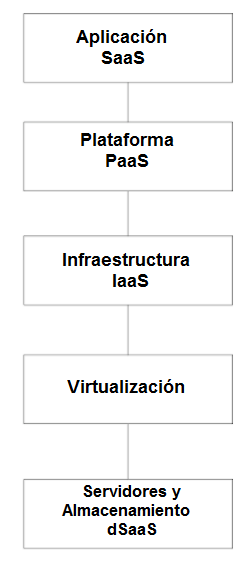
\includegraphics[width=.3\textwidth]{cloudcapas}
		\caption{Arquitectura en capas de computaci\'on cloud \cite{handbook}}
		\label{fig:capas1}
	\end{center}
\end{figure}
\begin{enumerate}[label=\alph*)]
    \item{IaaS:} Se refiere a los recursos informáticos como un servicio. Esto incluye computadoras virtualizadas con potencia de procesamiento garantizada y ancho de banda reservado para almacenamiento y acceso a Internet
    \item{PaaS:} Es similar a IaaS, pero también incluye sistemas operativos y servicios requeridos para una aplicación particular. En otras palabras, PaaS es IaaS con un stack de software personalizado para la aplicación dada.
    \item{SaaS:} Que se muestra en la parte superior de la figura \ref{fig:capas1}. SaaS permite a los usuarios ejecutar aplicaciones de forma remota desde la nube.
    \item{dSaaS:} Proporciona almacenamiento que el consumidor utilizar\'a, incluyendo los requisitos de ancho de banda para el almacenamiento.
\end{enumerate}
\end{justify}

\subsection{Seg\'un Tipo De Nube}
\begin{justify}
Hay tres tipos de computación cloud, los cuales se muestran en la figura \ref{fig:cloudtipos}
\begin{figure}[ht]
	\begin{center}
		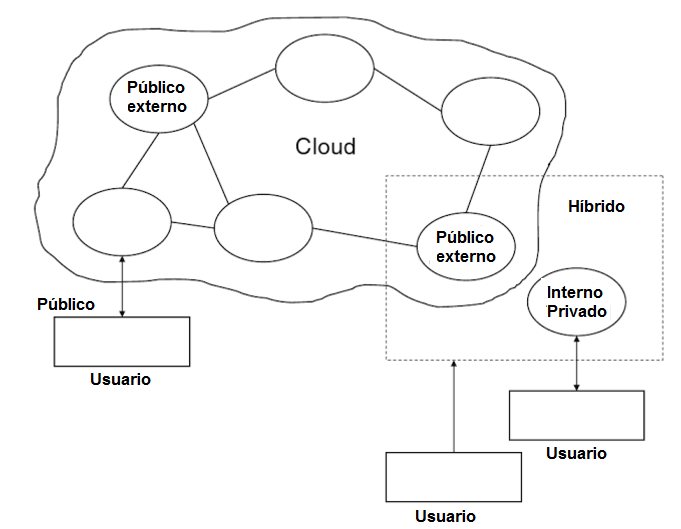
\includegraphics[width=.8\textwidth]{cloudtipos}
		\caption{Tres tipos de computaci\'on cloud \cite{handbook}}
		\label{fig:cloudtipos}
	\end{center}
\end{figure}
\begin{enumerate}[label=\alph*)]
    \item{P\'ublica:} En la nube pública (o en la nube externa), los recursos inform\'aticos se suministran din\'amicamente mendiante Internet a trav\'es de aplicaciones Web o Servicios Web de un proveedor externo (de terceros). Las nubes p\'ublicas son ejecutadas por terceros, y es probable que las aplicaciones de diferentes clientes se mezclen entre sí en los servidores, sistemas de almacenamiento y redes de la nube.
    \item{Privada:} La nube privada (o nube interna) se refiere a la computaci\'on cloud en redes privadas. Las nubes privadas se construyen para el uso exclusivo de un cliente, proporcionando un control total sobre los datos, la seguridad y la calidad del servicio. Las nubes privadas pueden ser construidas y administradas por la propia organización de TI de la empresa o por un proveedor de la nube.
    \item{H\'ibrida:} Un entorno de nube híbrido combina los modelos de nube pública y privada. Las nubes híbridas introducen la complejidad de determinar cómo distribuir aplicaciones a través de una nube pública y privada
    \item{Comunitaria:} El modelo de nube comunitaria permite el acceso a un número de organizaciones o consumidores que pertenecen a una comunidad y el modelo se construye para servir a algún propósito común y específico. Es para el uso de alguna comunidad de personas u organizaciones que comparten preocupaciones comunes en funcionalidades empresariales, requisitos de seguridad, etc. Este modelo permite compartir infraestructura y recursos entre múltiples consumidores pertenecientes a una única comunidad y por lo tanto se hace más barato comparado con una nube privada \cite{sandeep}
\end{enumerate}
\end{justify}

\subsection{Según Por Agentes Intervinientes En El Negocio}
\begin{justify}
Los agentes intervinientes en el negocio seg\'un \cite{tratecno}, se muestran en la figura \ref{fig:agentesintervinientes}
\begin{figure}[ht]
	\begin{center}
		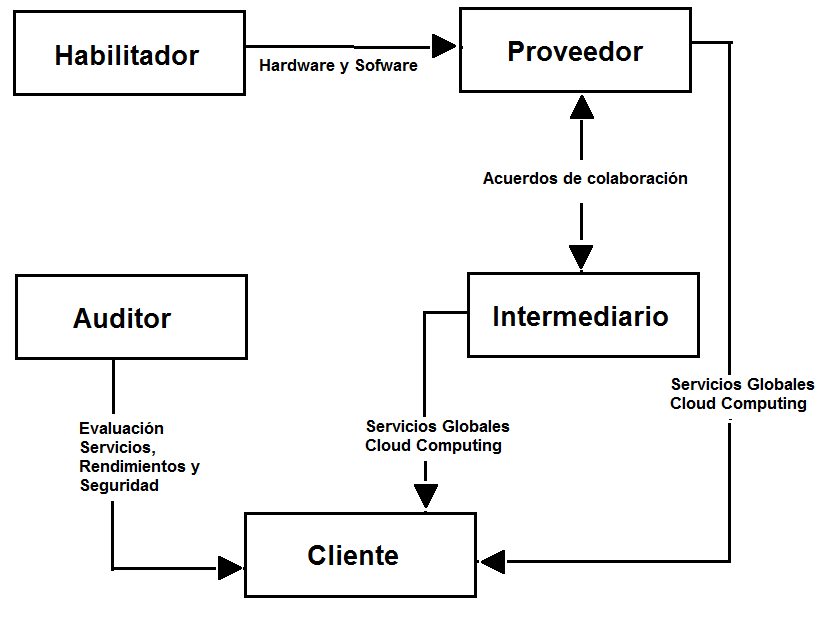
\includegraphics[width=.6\textwidth]{agentesintervinientes}
		\caption{Agentes intervinientes en el negocio \cite{tratecno}}
		\label{fig:agentesintervinientes}
	\end{center}
\end{figure}
\begin{enumerate}[label=\alph*)]
    \item{Habilitador:} Enfocados a ofrecer una serie de servicios Hardware o Software a otros proveedores.
    \item{Proveedor:} Los servicios que presta a los intermediarios y clientes, o bien los genera directamente el, o los contrata a otros proveedores o habilitadores.
    \item{Auditor:} Las funciones a desarrollar por los auditores, son las de llevar a cabo evaluaciones de los servicios, rendimientos y seguridad de las operaciones en el uso de las soluciones Cloud.
    \item{Intermediario:} Los intermediarios adecuan las soluciones para los clientes negociando los distintos servicios, añadiéndole en muchos casos ciertos servicios adicionales como pueden ser algunos apoyos en formación, implementación, etc.
    \item{Cliente:} Dentro del esquema de los agentes intervinientes, es aquel que va a contratar los servicios del resto de los agentes.
\end{enumerate}

\end{justify}

%%%%%%%%%%%%%%%%%%%%%%%%%%%% CAPITULO 2 %%%%%%%%%%%%%%%%%%%%%%%%%%%%
\vspace*{5em}
\chapter{VENTAJAS, DESVENTAJAS Y RETOS}
\vspace*{-2em}
\section{Ventajas}
\begin{justify}
Las soluciones y servicios de cloud computing ofrecen una serie de ventajas a las empresas privadas (econ\'omico-financieras,foco en el negocio, rapidez y flexibilidad, tecnol\'ogicas, seguridad, disponibilidad y movilidad, etc.), a la econom\'ia, a las organizaciones p\'ublicas y de investigaci\'on y a los ciudadanos (mayor y mejor oferta de servicios, gobierno abierto, educaci\'on), respecto de las funcionalidades ofrecidas por los sistemas tradicionales de TI y esto es gracias a su rapidez, flexibilidad, disponibilidad, etc. De entre todas las ventajas que hay, las más notables para los usuarios son el ahorro en costes y la facilidad para aumentar los recursos disponibles.
\\ Los ahorros en costes son debidos a que es posible evitar los gastos tanto en hardware, como en software, soporte y seguridad. Por otro lado, la flexibilidad y la escalabilidad de los recursos se hace de una manera muy sencilla y en el momento que el cliente lo requiera, de forma que puede aumentar o disminuir los recursos que está utilizando en cualquier momento y adem\'as pagando solo por lo que usa. Otra de las ventajas m\'as atrayentes es la capacidad de recuperación ante problemas, o desastres.
\\ Podemos decir que gracias a todas las ventajas que ofrece el paradigma del cloud computing frente a los m\'etodos tradicionales, est\'a haciendo que aumente la productividad de las empresas, se mejore en los servicios públicos y la calidad de vida.

\end{justify}
\newpage
\subsection{Ventajas para las empresas}
\begin{justify}
Actualmente el cloud computing es un instrumento acelerador para que una empresa logre evolucionar en su competividad proporcionando ventajas estrat\'egicas, t\'ecnicas, para la sostenibilidad y econ\'omicas que ya se mencionaron antes.
\begin{enumerate}[label=\alph*)]
    \item{Ventajas estrat\'egicas:} 
				\begin{itemize}
						\item{Creaci\'on de nuevos productos y servicios: } Esto es posible debido a la reduccio\'n de 	costes, que hace que sea posible que las empresas creen nuevos productos y/o servicios, que antes no resultaban rentables.
						\item{Trabajo colaborativo: } La computaci\'on en la nube permite que muchas personas a la vez puedan trabajar sobre la misma herramienta, aplicaci\'on o documento, de esta manera se fomenta la productividad, comunicaci\'on y colaboraci\'on entre empleados.
						\item{Mejora de la productividad: } Como los recursos est\'an disponibles para acceder a ellos desde cualquier ubicaci\'on f\'isica, se puede trabajar sobre los recursos de forma online, desde cualquier lugar, haciendo que aumente la flexibilidad de la empresa para trabajar a distancia y la productividad de sus empleados.
						\item{Innovaci\'on: } El ahorro en costes hace que la empresa pueda centrar sus esfuerzos en desarrollar su activadad de negocio, haciendo posible que la empresa tenga m\'as posibilidades de invertir en innovaci\'on.
				\end{itemize}
		\newpage
    \item{Ventajas te\'cnicas:}
				\begin{itemize}
						\item{}La nube es una plataforma que permite a los usuarios disponer de la tecnolog\'ia m\'as actual, lo que hace que no haya riesgo de p\'erdida de competitividad por obsolescencia tecnol\'ogica. Adem\'as de esto el tiempo de adopci\'on de nuevos servicios, infraestructuras o tecnolog\'ias es mucho menor. 
						\item{}Los proveedores de cloud computing tambi\'en ofrecen soporte y redundancia en los sistemas que sus clientes contratan, de manera que existe una gran resistencia a desastres y buena capacidad de recuperación ante fallos.
				\end{itemize}
    \item{Ventajas para la sostenibilidad:} 
				\begin{itemize}
						\item{}La reducción en el consumo de energ\'ia es notable, debido a que la empresa necesita de menos equipamiento propio, ya que lo contrata al proveedor. Esto es posible porque la empresa no dispone de un exceso de recursos inform\'aticos, sino que la plataforma que contrata se adapta a las necesidades de su entidad. Los centros de datos utilizan diseños de infraestructuras avanzados, de forma que los sistemas de refrigeraci\'on y de acondicionamiento de energ\'ia se aprovechen bien y no haya p\'erdidas.
				\end{itemize}
\end{enumerate}
\end{justify}
\newpage
\subsection{Ventajas para la econom\'ia}
\begin{justify}
El cloud computing genera un notable efecto de dinamizaci\'on econ\'omica y del empleo en aquellos pa\'ises en los que su desarrollo e implantaci\'on est\'a m\'as evolucionado. Al igual que el sector TIC o la aparici\'on de Internet gener\'o una revoluci\'on de los modelos empresariales y econ\'omicos durante las tres \'ultimas d\'ecadas y supuso un motor de desarrollo para todos los pa\'ises, el cloud computing est\'a llamado a ser un nuevo punto de ruptura para la econom\'ia mundial en general y para el sector de las tecnolog\'ias y servicios profesionales en particular.
\\ Este efecto dinamizador se fundamenta en el hecho de que los beneficios que obtienen las empresas proveedoras de servicios cloud se reinvierte en la econom\'ia a trav\'es de consumos intermedios en otros sectores derivados, genera una dinamizaci\'on de empleo cualificado e incrementa el poder adquisitivo y el consumo en un territorio. 
\\ Adicionalmente, las empresas suscriptoras del servicio adquieren las econom\'ias de escala de los proveedores, reduciendo con ello sus costes globales en TI. Gracias a la presencia de estas econom\'ias de escala en el sector, se suprimen las barreras de entrada en el mercado de nuevos proveedores, suscriptores e intermediarios, dinamizando la econom\'ia y promoviendo la aparición de nuevos modelos de negocio, productos y servicios y facilitando la creación de nuevas empresas y empleo.
\\ Estas econom\'ias de escala también favorecen la sostenibilidad de las empresas de nueva creación que pueden dedicar todos sus esfuerzos a su negocio y reducir el riesgo de "morir de \'exito"\hspace{0.1cm}por no poder escalar adecuadamente ante situaciones de demanda superior a las expectativas. Es evidente que esta ventaja resulta de especial trascendencia para las pequeñas y medianas empresas.
\\ Adicionalmente, la mayor eficiencia en el uso de la infraestructura TI permite ahorros energ\'eticos significativos con la consiguiente mejora en el impacto medioambiental, añadiendo a los atractivos de las tecnolog\'ias cloud computing el de ser respetuosas con el medio ambiente

\end{justify}
\newpage
\subsection{Ventajas para las administraciones p\'ublicas}
\begin{justify}
Una administraci\'on p\'ublica es similar en muchos aspectos a una empresa privada, ya que ambas lo que buscan es prestar servicios, gestionar recursos, relacionarse con los proveedores, etc. Entonces, es lógico pensar que estas entidades tambi\'en pueden optar por una soluci\'on cloud para desempeñar su actividad y as\'i beneficiarse de las ventajas que ofrece esta tecnolog\'ia.

Adem\'as de las ventajas obvias que este paradigma aporta a este tipo de entidades, tales como el ahorro en costes tecnol\'ogicos, la flexibilidad y la escalabilidad, el ahorro energ\'etico, existen otras muchas ventajas espec\'ificas para las administraciones p\'ublicas:
				\begin{itemize}
						\item{}Facilita las tareas de soporte tecnol\'ogico intensivo, ya que es el proveedor el que se encarga de esto y por lo tanto no se incurre en grandes gastos en este aspecto.
						\item{}Generalizaci\'on de todos los servicios transversales de la Administraci\'on y por lo tanto un aprovechamiento y reutilizaci\'on de las infraestructuras tecnol\'ogicas.
						\item{}Modernizaci\'on de entidades pequeñas, locales o municipales, que no disponen
de recursos necesarios para modernizar sus procesos y equipos de la forma tradicional.
						\item{}Investigaci\'on y colaboraci\'on en entidades con car\'acter educativo, tales como universidades, fundaciones, centros de investigaci\'on, etc. Incluso la cooperaci\'on entre estos centros.
				\end{itemize}
\end{justify}
\newpage
\subsection{Ventajas para la investigaci\'on cient\'ifica}
\begin{justify}
Es totalmente esencial que exista un ambiente de colaboraci\'on e interoperabilidad entre entidades dedicadas a la investigaci\'on, adem\'as de la existencia de tecnolog\'ias avanzadas, por lo que la nube, tanto privada como p\'ublica, puede favorecer en muchos aspectos al desarrollo de estas actividades.
Algunas de las ventajas m\'as notables del cloud computing en estas \'areas son las siguientes:
				\begin{itemize}
						\item{}Plataformas de colaboraci\'on entre entidades, de manera que la realizaci\'on de investigaciones y proyectos de forma conjunta es mucho m\'as r\'apida y eficaz.
						\item{}Estandarizaci\'on de sistemas, procesos y datos entre empresas que participan
en el mismo proyecto.
						\item{}Disposici\'on de entornos grandes e intensivos de procesamiento de datos, de manera que las tareas se realicen m\'as ágilmente y ahorrando en costes.
				\end{itemize}
\end{justify}
\newpage
\subsection{Ventajas para los ciudadanos}
\begin{justify}
Gracias a la tecnolog\'ia cloud ahora es posible acceder a la informaci\'on desde cualquier localizaci\'on.Las caracter\'isticas de este paradigma no son visibles para los usuarios, pero gracias a ellas, son capaces de acceder a gran variedad de servicios de forma gratuita o a precios muy bajos y lo m\'as importante, sin necesidad de disponer de equipos especializados para ello. Algunos de estos servicios más t\'ipicos y conocidos son los gestores de correo electr\'onico, buscadores, enciclopedias, \'albumes de fotograf\'ias, etc.
Entre las principales ventajas para los ciudadanos, que aporta la computaci\'on cloud tenemos:
				\begin{itemize}
						\item{}Amplia oferta de servicios y productos tecnol\'ogicos similares, debido a la competitividad existente, que permite a los ciudadanos poder elegir entre las soluciones que le parecen m\'as estables, econ\'omicas y seguras.
						\item{}Variedad en los servicios disponibles para que los ciudadanos realicen sus tareas cotidianas, desde ocio, hasta trabajo, gesti\'on del hogar, educaci\'on, etc. Gracias a los dispositivos m\'oviles, la utilizaci\'on de estos servicios es mucho m\'as sencilla.
						\item{}Los ciudadanos pueden acceder a un mayor n\'umero de servicios, gracias a la administración electr\'onica. Lo hacen a trav\'es de Internet y de esta forma pueden realizar de manera m\'as sencilla, \'agil y efectiva muchos tr\'amites de la administraci\'on.
						\item{}Disponibilidad de un "gobierno abierto"\hspace{0.1cm}que permita que los ciudadanos puedan acceder a la informaci\'on sobre las actividades realizadas por el gobierno, sus gastos, datos que genera, etc. Además de fomentar la participaci\'on ciudadana para diseñar pol\'iticas p\'ublicas.
						\item{}Las redes sociales permiten que los ciudadanos compartan experiencias, conocimientos, que hagan negocios o que demanden bienes y servicios.
				\end{itemize}
\end{justify}
\newpage
\section{Desventajas}
\begin{justify}
Junto a los beneficios tambi\'en existen ciertas desventajas o riesgos expuestos por los
detractores de esta tecnolog\'ia y que nos recomiendan no confiar toda la informaci\'on de nuestra empresa a la Nube.
Entre las principales desventajas tenemos:
				\begin{itemize}
						\item{}El problema de la estabilidad de la conexi\'on a Internet. Los detractores dudan de que la velocidad de conexi\'on y la estabilidad proporcionada por los ISP sea suficiente para gestionar el volumen de datos generado por el n\'umero de empresas que se sumen a la Nube. 
						\item{} Tener nuestra informaci\'on y su gesti\'on a la Nube significa perder el control sobre ella y si el proveedor de servicios de la Nube tiene un problema a la hora de suministrar, \'este se traduce autom\'aticamente en la imposibilidad de acceder a nuestros datos y, por tanto, de trabajar. Si el tiempo es oro para nuestro negocio, confiar en la Nube puede ser lo menos aconsejable.

						\item{}Otro problema es el de la seguridad. Por ejemplo, aquella informaci\'on extremadamente confidencial o delicada y que se encuentre en la Nube en manos de terceros en quienes confiamos que hagan un buen trabajo a la hora de asegurarla y protegerla, pero si no es as\'i, los grandes perjudicados seremos nosotros, lo mismo se puede aplicar para aquella información privada de los empleados de una empresa. Hoy en d\'ia se esta acostumbrado a que los empleados usen los recursos de la empresa (Servidores, conexi\'on a Internet, etc.) para gestiones privadas y esa misma privacidad podr\'ia ser amenazada si esos datos se encuentran almacenados en un sitio controlado por otros. 
				\end{itemize}
				
En definitiva, debemos reflexionar tanto las ventajas como las desventajas y compararlas con las necesidades espec\'ificas del negocio actual. Si nos preocupa sobre todo el presupuesto, la Nube puede ser una buena opci\'on a considerar; pero si, por el contrario, nuestra mayor preocupaci\'on es la seguridad y protecci\'on de nuestra informaci\'on, la Nube está todavía muy lejos de ser considerada como alternativa viable.
\newpage
El volumen de datos tambi\'en es un delimitador para saber si una pequeña o mediana empresa est\'a preparada para ser elevada a la Nube. Cuanto mayor sea el volumen de informaci\'on que procesamos y
almacenamos, menos recomendable será confiar en la computación en nube. Algunas soluciones intermedias podria ser subir a la Nube s\'olo una parte de nuestra informaci\'on; aquella, por ejemplo, que precise ser accesible desde m\'ultiple localizaciones. Y el resto, la m\'as sensible, almacenarla y gestionarla desde sistemas propios.
\end{justify}
\newpage
\section{Retos}
\subsection{Disponibilidad del servicio}
\subsection{Restricciones geogr\'aficas}
\subsection{Seguridad y privacidad de datos}
\subsection{Amortizaci\'on tecnol\'ogica}
%%%%%%%%%%%%%%%%%%%%%%%%%%%% CAPITULO 3 %%%%%%%%%%%%%%%%%%%%%%%%%%%%
\vspace*{5em}
\chapter{TITULO DEL CAPITULO 3}
\vspace*{-2em}
\begin{justify}
Holaque hace como esta muy bien esxop me legr qurbfgs tu vida hace triempo bla bla bla bla bla xd xd xd d
\end{justify}

%%%%%%%%%%%%%%%%%%%%%%%%%%%% CAPITULO 4 %%%%%%%%%%%%%%%%%%%%%%%%%%%%
\vspace*{5em}
\chapter{TECNOLOG\'IAS ACTUALES}
\vspace*{-2em}

Claramente la nube se est\'a convirtiendo en una plataforma de innovaci\'on y transformaci\'on general.
\\ Actualmente muchas empresas de todo el mundo est\'an ofreciendo una amplia gama de servicios en la nube, la abundancia puede ser abrumadora.
 
\section{Empresas que brindan servicios de Cloud}
\subsection{Amazon.com}
\begin{justify}
{\bf{Amazon Web Services (AWS)}} es una plataforma de servicios en la nube que ofrece potencia de c\'omputo, almacenamiento de bases de datos, entrega de contenido y otra funcionalidad para ayudar a las empresas a escalar y crecer. \citep{aws}

AWS se encuentra detrás del \'exito de muchas compañías, startups y sector p\'ublico, como: 
\begin{itemize}
	\item  \textbf{Netflix:} AWS permite a Netflix desplegar rápidamente miles de servidores y terabytes de almacenamiento en cuesti\'on de minutos. Los usuarios pueden ver programas y películas de Netflix desde cualquier parte del mundo, incluso en la web, en tabletas o en dispositivos móviles como el iPhone.\citep{awscasos}
	\item  \textbf{Spotify:}	Debido a que el objetivo de la compañía es ayudar a la gente a escuchar cualquier música que quieran, cuando quieran, Spotify se enfrenta al desaf\'io de catalogar no sólo ayer y las canciones populares de hoy, sino también todas las que se publicarán en el futuro. Spotify agrega más de 20.000 pistas al día a su catálogo. \\	
La  compa\~{n}\'ia cre\'o sistemas basados en Python para interactuar con su enorme volumen de contenido en Amazon S3. Además, Amazon CloudFront entrega la aplicación Spotify y las actualizaciones de software a los usuarios. \\ Al igual que las tendencias musicales cambian continuamente, Amazon Web Services (AWS) ayuda a Spotify a evaluar continuamente su infraestructura para cumplir con los objetivos de negocio en constante evoluci\'in.\citep{awscasos}
	\item  \textbf{Adobe:}Adobe utiliza AWS para proporcionar ambientes operativos de varios terabytes para sus clientes. Al integrar sus sistemas con AWS Cloud, Adobe puede centrarse en implementar y operar su propio software en lugar de infraestructura.\citep{awscasos}
\end{itemize}
De acuerdo con \cite{awscasos} otras  de las empresas que cuentan con el respaldo de AWS son  Dunkin Donuts, Airbnb, Kellogs, Siemens, BCP, Johmson-Johmson, etc. 
\\Actualmente la nube de AWS funciona en 44 zonas de disponibilidad dentro de 16 regiones geogr\'aficas del mundo, con planes anunciados para crear 14 zonas m\'as y cinco regiones adicionales en China, Francia, Hong Kong, Suecia y una segunda regi\'on AWS GovCloud en los EE.UU. \citep{aws}

\begin{figure}[ht]
\begin{center}
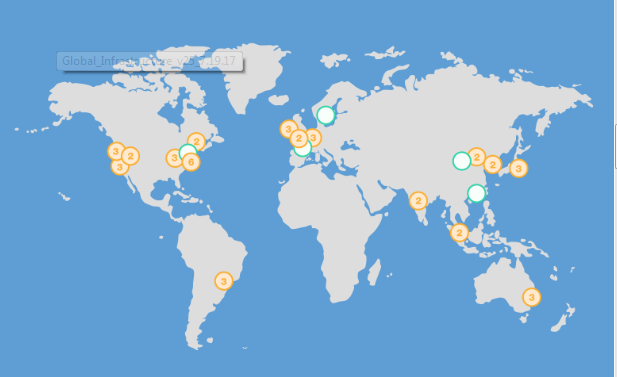
\includegraphics[scale=0.8]{aws_paises}
\end{center}
\begin{center}
\vskip -0.5cm
\caption{\small{Distribución de AWS.}}
{\small{Fuente: \cite{aws}}}
\end{center}
\end{figure}

\end{justify}
\subsection{Google Inc}
\begin{justify}
{\bf Google Cloud Plataform} consiste en un conjunto de servidores d f\'isico as\'i como virtuales que est\'an contenidos en los centros de datos de Google alderedor del mundo.
\\ Google cuenta con el modo de despliegue  multi regional Google Cloud Plataform, lo cual permite al usuario elegir el centro de datos para sus aplicaciones.
\end{justify}
\begin{figure}[ht]
\begin{center}
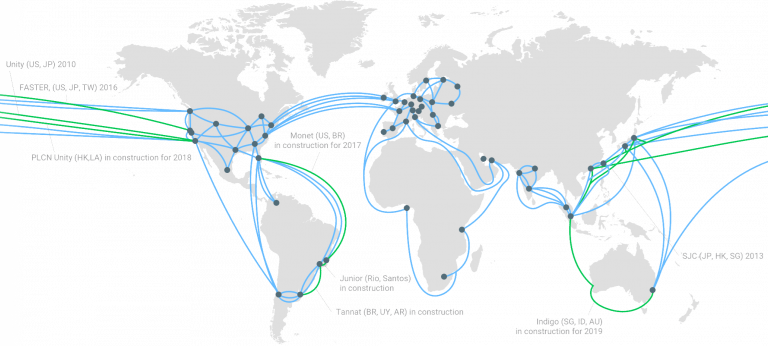
\includegraphics[scale=0.6]{google_cloud}
\end{center}
\begin{center}
\vskip -0.5cm
\caption{\small{Red de Google Cloud Platform.}}
{\small{Fuente: \cite{google_cloud}}}
\end{center}
\end{figure}
\begin{justify}
Según \cite{google_cloud} en las \'ultimas encuestas de SADA Systems sobre el uso p\'ublico de la nube, los  gerentes de TI encuestados dan se\~{n}ales del crecimiento que esta teniendo hoy en día la infraestructura de nube p\'ublica.
\end{justify}
\begin{figure}[ht]
\begin{center}
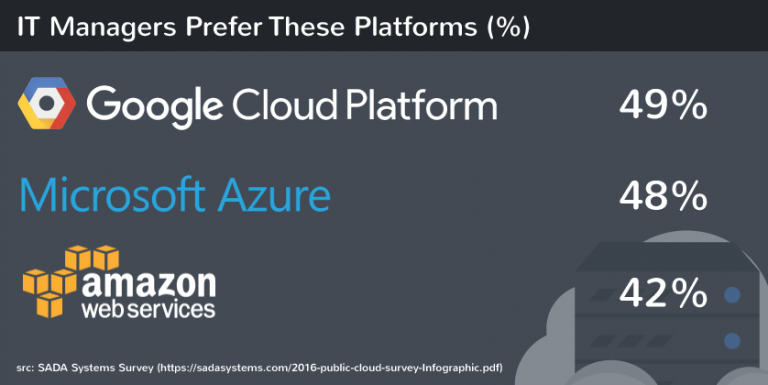
\includegraphics[scale=0.4]{encuesta}
\end{center}
\begin{center}
\vskip -0.5cm
\caption{\small{Resultados de Encuesta sobre el uso de nubes p\'ublicas}}
{\small{Fuente: \cite{google_cloud}}}
\end{center}
\end{figure}

Estas son algunas de las empresas que  desarrollan sus productos con Google Cloud Platform:
\begin{itemize}
	\item \textbf{Pocket Gems:} Utiliza App Engine para procesar cientos de miles de jugadores m\'oviles en tiempo real.
	\item \textbf{Khan Academy :}Khan Academy usa Google Cloud Platform para poner cursos gratuitos y de gran calidad al alcance de todos.
	\item \textbf{Coca-Cola:} Comprueba cómo está utilizando Google Cloud Platform Coca-Cola para estar a la altura de los eventos deportivos más grandes del mundo.
	\item \textbf{Atomic Fiction:} Crea efectos especiales para las series de televisión y las películas más importantes del mundo, gracias a los potentísimos recursos informáticos de Google Cloud Platform.
\end{itemize}
\begin{justify}
Un gran punto a favor que tiene hoy en día Google Cloud Plataform es que permite la migraci\'on en vivo de m\'aquinas Virtuales, funcionalidad que ni Azure ni AWS tienen. En la siguiente figura se detallan los  pasos de alto nivel involucrados en una migración de VM en vivo (Figura \ref{migracion}).
\end{justify}
\FloatBarrier 
\begin{figure}[ht]
\begin{center}
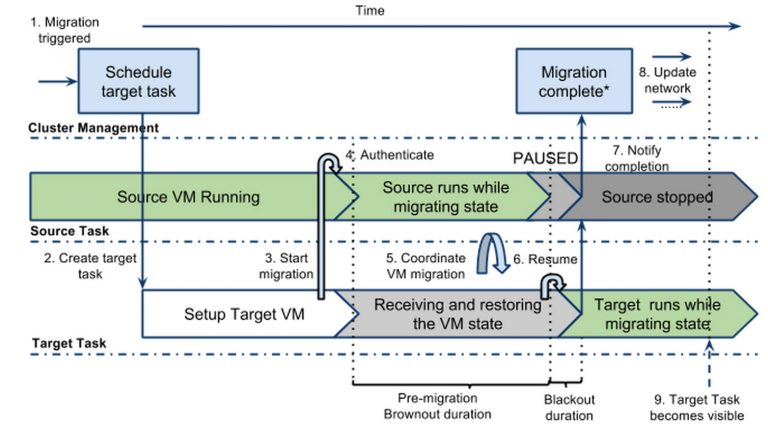
\includegraphics[scale=0.7]{migracion}
\end{center}
\begin{center}
\vskip -0.5cm
\caption{\small{ Pasos de alto nivel involucrados en una migraci\'on de VM en vivo}}
\label{migracion}
{\small{Fuente: \cite{google_cloud_migration}}}
\end{center}
\end{figure}

\subsection{Azure}
\begin{justify}
Microsoft Azure es una creciente colección de servicios en la nube integrados que los desarrolladores y los profesionales de TI utilizan para crear, implementar y administrar aplicaciones a través de nuestra red global de centros de datos. Con Azure, obtiene la libertad de crear e implementar donde quiera, utilizando las herramientas, las aplicaciones y los marcos que prefiera.\citep{azure_def}

Estas son algunas de las empresas que  desarrollan sus productos con Microsoft Azure:
\begin{itemize}
	\item \textbf{Carviresa :} Para mejorar la planificación y gestión de sus recursos, y centralizar los datos de negocio procedentes de sus tres ubicaciones.
	\item \textbf{Guzman Global :}La multinacional española ha elegido Microsoft Dynamics CRM Online por su usabilidad, escalabilidad y sus altos estándares de seguridad en la nube, factores que le permiten replicar su modelo fácilmente en diferentes países.
	\item \textbf{NAE :} Para mejorar su gestión comercial con la ayuda del partner Innovar Tecnologías.
\end{itemize}

\end{justify}

\section{Casos de Implementación}
	\begin{justify}
	A continuación se presentarán  las diferentes que empresas o instituci\'on que aplicaron las buenas pr\'acticas en la implementaci\'on de diferentes soluciones cloud (Tabla \ref{tablaEmpresas}) , casos pertenecientes a diferentes ramas, actividad económica, administración publica, etc.
	\end{justify}

	\begin{table}[ht]		
		\centering
		\caption{Casos de \'Exito implementando Cloud Computing}
		\label{tablaEmpresas}
		\begin{tabular}{|p{4.2cm} |p{2.3cm} |p{2.5cm} |p{4cm}|} \hline
			\bf{Sector} & \bf{Proveedor} & \bf{Modelo de Negocio} & \bf{Empresa o Institución} 
			\\ \hline \hline
			Adminitraci\'on P\'ublica & Microsoft & SaaS &  Generalitat de Catalunya 
			\\ \cline{2-4}
			 & CIPSA y REGTSA & SaaS (cloud privada) & CIPSA y REGTSA  
			\\ \hline
			Audio Visuales  & Spotify & SaaS & AWS
			\\ \hline
			Correo electr\'onico & Amazon & PaaS / IaasS & AWS
			\\ \hline
			Inform\'atica y telecomunicaciones & Annova y Pixelware & PaaS & Proyecto PymeCloud 
			\\ \cline{2-4}
			 & EyeOS & PaaS & EyeOS  
			\\ \cline{2-4}
			 & Arsys & SaaS / PaaS / IaaS & EyeOS  
			\\  \cline{2-4}
			 & Fresh Books & SaaS & Fresh Books  
			\\  \hline
			Ivestigaci\'on, desarrollo y manufactura & Windows Azure & PaaS & 3M 
			\\ \hline
			Ivestigaci\'on Biom\'edica & VORTAL & SaaS & Organismo P\'ublico de España 
			\\ \hline
			Medios de Comuniaci\'on & NTS y Salesforce.com & SaaS & Grupo Vocento \\ \hline
			Transporte & Estudio Cero & SaaS & Estudio Cero\\ \hline 
		\end{tabular}
		\vskip 0.2cm
		\begin{center}
			{\small{Fuente: Elaboraci\'on Propia - \cite{Ferrari}.}}
		\end{center}
	\end{table}



\section{Diferencias entre Empresas que ofrecen Cloud Computing}
	\begin{justify}
	Seg\'un \cite{Akami} las empresas de Cloud Computing se diferencian seg\'un:
	\begin{enumerate}[label=\alph*)]
		\item \textbf{Tipo de servicio ofrecido: } En la nube existen diferentes tipos de servicio (v\'ease cap. \ref{cap1}. La entidad que se quiera contratar debe definir muy bien cu\'ales ser\'an los Acuerdos de Nivel de Servicio (SLA) que mejor se ajusten a las necesidades.
		\item \textbf{La escala y resistencia de la arquitectura:} Las mejores empresas de cloud computing tienen varios centros de datos dispersos geográficamente, lo que garantiza la disponibilidad ininterrumpida del servicio para sus cliente.
		\item \textbf{Calidad del componente de autoservicio:} La administraci\'on  de los servicios en la nube se realiza por un portal web, por ello, el portal debe contar con ciertas normas y permitir el control f\'acil del servicio.
		\item \textbf{Longevidad y experiencia:} Seg\'un \cite{CristianCA} en el 2012  el modelo de cloud computing se encontraba en etapa de desarrollo, por ese motivo existían pocas empresas que apostaban por el modelo; sin embargo,  en la actualidad existen cada día mas empresas ofreciendo este modelo, este es el motivo por el que cual al momento de querer adquirir los servicios que ofrece se debe tener en cuenta la experiencia, pues muchas son nuevas y no han sido probadas.
	\end{enumerate}
	Si desea conocer algunas recomendaciones para contratar servicios en la nube revise el documento de \cite{Beimar}
\end{justify}


%%%%%%%%%%%%%%%%%%%%%%%%%%%%%%%%%%%%%%%%%%%%%%%%%%%%%%%%%%%%%%%%%%%%%%%%%%%


\newpage
%%%%%%%%%%%%%%%%%%%%%%%%%%%% CONCLUSIONES %%%%%%%%%%%%%%%%%%%%%%%%%%%%
\addcontentsline{toc}{chapter}{Conclusiones}
\vspace*{6em}
\begin{center}
{\bf{\large{\underline{CONCLUSIONES}}}}
\end{center}
\begin{justify}
Podemos concluir muchas cosas v:
\end{justify}
%%%%%%%%%%%%%%%%%%%%%%%%%%%%%%%%%%%%%%%%%%%%%%%%%%%%%%%%%%%%%%%%%%%%%%%%%%%



%%%%%%%%%%%%%%%%%%%%%%%%%%%% BIBLIOGRAFIA %%%%%%%%%%%%%%%%%%%%%%%%%%%%
\addcontentsline{toc}{chapter}{Bibliograf\'ia}
\vspace*{6em}
 \bibliography{Bibliografia}
%%%%%%%%%%%%%%%%%%%%%%%%%%%%%%%%%%%%%%%%%%%%%%%%%%%%%%%%%%%%%%%%%%%%%%%%%%%



\end{document}
